\documentclass{beamer}

\usepackage{tikz}
\usetikzlibrary{arrows,automata,positioning,fit,calc,shadows}

\usepackage{minted}
\usemintedstyle{friendly}
\setminted{
  breaklines=true,
  samepage=true,
}

\usepackage[english]{babel}
\usepackage[backend=biber,style=numeric-comp,sorting=none]{biblatex}
\addbibresource{/Users/brucecollie/Documents/Uni/Academic/zotero.bib}

\title{Statically Checked Assertions for TESLA}
\author{Bruce Collie}
\subject{Part III Computer Science}

\AtBeginSection[]
{
  \begin{frame}
    \tableofcontents[currentsection]
  \end{frame}
}

\begin{document}

\frame{\titlepage}

\begin{frame}
  \tableofcontents
\end{frame}

\section{Background}

\begin{frame}
  \frametitle{Temporal Properties}

  \begin{itemize}
    \item Traditional debugging assertions are limited in scope
      \begin{itemize}
        \item Current stack frame
        \item Global state
        \item What is happening \emph{right now}?
      \end{itemize}
    \item More interesting properties are often temporal
      \begin{itemize}
        \item What happened in the past?
        \item What happens in the future?
      \end{itemize}
    \item Theoretical approach: logics like LTL, CTL etc.
  \end{itemize}
\end{frame}

\begin{frame}[fragile]
  \frametitle{TESLA}
  \framesubtitle{\textbf{T}emporally \textbf{E}nhanced \textbf{S}ystem
  \textbf{L}ogic \textbf{A}ssertions}

  \begin{itemize}
    \item Applies temporal logic assertions to large C programs
      \begin{itemize}
        \item FreeBSD
        \item OpenSSL
        \item GNUStep
      \end{itemize}

    \item Implemented as an LLVM-based toolchain

    \item Assertions are checked at run time
  \end{itemize}

  \begin{center}
    \begin{minipage}{0.5\textwidth}
      \begin{minted}[mathescape,
        fontsize=\footnotesize,
        framesep=2mm]{c}
TESLA_WITHIN(main, eventually(
  foo(ANY(ptr)) == 0,
  call(bar) || call(baz)
));
      \end{minted}
    \end{minipage}
  \end{center}
\end{frame}

\section{Why static analysis?}

\begin{frame}
  \frametitle{Performance}

  \begin{itemize}
    \item TESLA instrumentation is expensive
      \begin{itemize}
        \item 2.4$\times$ as many instructions executed
        \item Reaching an assertion runs extra code
        \item Startup and shutdown costs
        \item Too slow for production builds
      \end{itemize}

    \item Temporal bounds improve things a little

    \item If an assertion is \textbf{always} true, we don't need to run it
      \begin{itemize}
        \item Prove assertions at compile time
        \item If we can, instrumentation code can be removed
      \end{itemize}
  \end{itemize}
\end{frame}

\begin{frame}
  \frametitle{Other Benefits}

  \begin{itemize}
    \item Better understanding of assertions
      \begin{itemize}
        \item In what circumstances can they fail?
        \item Counterexample generation
      \end{itemize}

    \item ``Engineering'' improvements
      \begin{itemize}
        \item Bug fixes
        \item LLVM upgrades
        \item Documentation refresh
      \end{itemize}
  \end{itemize}
\end{frame}

\section{Model Checking TESLA}

\begin{frame}
  \frametitle{Bounded Model Checking}

  \begin{itemize}
    \item Does a program satisfy a specification?
      \begin{itemize}
        \item Find counterexamples to its negation
        \item ...with an upper bound on length
      \end{itemize}
    \item Generates minimal counterexamples
    \item Potentially unsound
  \end{itemize}
\end{frame}

\begin{frame}
  \frametitle{TMC}
  \framesubtitle{\textbf{T}ESLA \textbf{M}odel \textbf{C}hecker}

  \begin{itemize}
    \item Bounded model checker for TESLA
    \item Uses LLVM to transform a program to a checkable form
      \begin{itemize}
        \item Inlining, event identification, argument mapping
      \end{itemize}
    \item Constructs a finite automata
      \begin{itemize}
        \item Accepts or rejects possible program executions
      \end{itemize}
    \item SMT solver used for data flow checking
      \begin{itemize}
        \item Infers function return values for a potential execution
      \end{itemize}
    \item Produces a counterexample if assertion not always true
  \end{itemize}
\end{frame}

\begin{frame}
  \begin{center}
    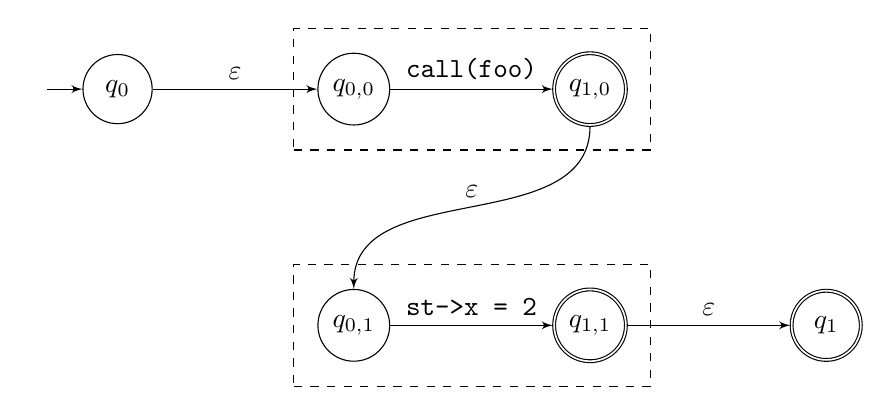
\begin{tikzpicture}[>=latex',initial text={},
                        node distance=3cm,on grid,auto]
      \node[state,initial] (realstart) [] {$q_0$};
      \node[state] (start) [right=of realstart] {$q_{0,0}$};
      \node[state,accepting] (end) [right=of start] {$q_{1,0}$};

      \node[state] [below=of start] (start2) {$q_{0,1}$};
      \node[state,accepting] [right=of start2] (end2) {$q_{1,1}$};

      \node[draw,dashed,fit=(start) (end), inner sep=0.3cm] {};
      \node[draw,dashed,fit=(start2) (end2), inner sep=0.3cm] {};

      \node[state,accepting] [right=of end2] (realend) {$q_1$};

      \path[->] (start) edge node {\texttt{call(foo)}} (end);
      \path[->] (start2) edge node {\texttt{st->x = 2}} (end2);

      \path[->] (realstart) edge node {$\varepsilon$} (start);
      \path[->] (end2) edge node {$\varepsilon$} (realend);
      \draw[->,out=270,in=90] (end.south) to node[above]{$\varepsilon$} (start2.north);
    \end{tikzpicture}
  \end{center}
\end{frame}

\section{Using TESLA and TMC}

\begin{frame}
  \frametitle{lwIP}
  \framesubtitle{\textbf{L}ight\textbf{w}eight \textbf{IP}}

  \begin{itemize}
    \item What can TESLA / TMC be used for in practice?
    \item Original aim was to instrument a TCP implementation
      \begin{itemize}
        \item lwIP is a widely used implementation of TCP/IP
        \item Validate its internal state machine
      \end{itemize}
    \item Source code features make instrumentation hard
      \begin{itemize}
        \item Macros, function pointers, coding style
      \end{itemize}
    \item TESLA works best at API boundaries
  \end{itemize}
\end{frame}

\begin{frame}
  \frametitle{Echo Server}

  \begin{itemize}
    \item Instrumented existing application with TESLA
    \item Assertions on TCP API boundary
      \begin{itemize}
        \item Validating usage of API methods
        \item Properties given informally in documentation
      \end{itemize}
    \item Process is general
  \end{itemize}
\end{frame}

\section{Results}

\begin{frame}
  \frametitle{Performance}

  \begin{itemize}
    \item lwIP app is much slower when instrumented
      \begin{itemize}
        \item Bulk transfer benchmark of the echo server
        \item 60\% relative throughput
      \end{itemize}
    \item TMC improved performance to 84\%
    \item Special-cased optimisation removes all overhead
      \begin{itemize}
        \item If all assertions are provable
      \end{itemize}
    \item Running TMC is \emph{slow}
      \begin{itemize}
        \item Overnight for largest existing assertion corpus
        \item Only slow if no counterexamples exist
      \end{itemize}
  \end{itemize}
\end{frame}

\begin{frame}
  \frametitle{Correctness}

  \begin{itemize}
    \item TMC aims for \emph{soundiness}
    \item False positives are much worse than false negatives
    \item Able to prove useful properties about data structures
      \begin{itemize}
        \item Progress properties of mutex locks
      \end{itemize}
    \item Test suite implemented as part of development
  \end{itemize}
\end{frame}

\section{Future Work and Conclusions}

\begin{frame}
  \frametitle{Future Work}

  \begin{itemize}
    \item Improved usability
    \item Wider distribution in the real world
    \item Model checker performance
    \item More expressive assertions
  \end{itemize}
\end{frame}

\begin{frame}
  \frametitle{Conclusions}

  \begin{itemize}
    \item It's possible to do static analysis
      \begin{itemize}
        \item Assertions are easily expressed as automata
        \item TMC can check a useful subset of TESLA
      \end{itemize}
    \item It's worth doing static analysis
      \begin{itemize}
        \item Big performance gains available
        \item Makes TESLA more widely applicable
      \end{itemize}
    \item It's sometimes hard to use TESLA on existing code
      \begin{itemize}
        \item ...but can be useful at API boundaries
        \item Much easier to write code with TESLA in mind
      \end{itemize}
    \item There's a lot to work on!
  \end{itemize}
\end{frame}

\begin{frame}[c]

  \begin{center}
  \Huge Questions
  \end{center}

\end{frame}

\end{document}
